% Multi-Agent Artificial Intelligence Group Project
% Coursework 1 - Real-time advertising bidding strategy
% Author: Wenjie Boon / Aisha Aldosery / Hend Almalik 

\documentclass{sig-alternate-05-2015}
\usepackage{siunitx}
\usepackage{graphicx}
\usepackage{adjustbox}
\usepackage{amsmath}
\usepackage{textcomp}
\usepackage{subfig}
 
\graphicspath{ {./images/} }

\makeatletter
\def\@copyrightspace{\relax}
\makeatother


\begin{document}

% Copyright
\setcopyright{acmcopyright}

\title{COMP0124 Multi-Agent Artificial Intelligence Group Project}
\subtitle{Real-Time Bidding Strategy - Team 10}

\numberofauthors{3} 

\author{
% 1st. author
\alignauthor
Wenjie Boon\\
       \affaddr{University College London}\\
       \email{wenjie.boon.18@ucl.ac.uk}
% 2nd. author
\alignauthor
Aisha Aldosery\\
       \affaddr{University College London}\\
       \email{a.aldosery@ucl.ac.uk}
% 3rd. author
\alignauthor
Hend Almalik\\
       \affaddr{University College London}\\
       \email{hend.almalik.18@ucl.ac.uk}
}

\date{11 March 2019}

\maketitle
\begin{abstract}
Real-time bidding (RTB) is the auctioning of online advertising impressions that occurs whenever a user loads a webpage containing advertising slots serviced by ad-exchanges. For every auction, advertisers will be provided a myriad of information such as page information and user details, this will then be used by the advertisers to determine how much they are willing to bid for the impression.

In this project, we explore different bidding strategies in both single and multi-agent environments, with the objective of maximising clicks from a set of advertising impressions. We explored bidding strategies in a single agent environment, evaluating basic strategies such as constant and random bidding, before implementing more efficient strategies that use click-through-rate classifiers such as linear and non-linear bidding. Finally, we put everything together and implement a bidding strategy that will be useful in a multi-agent environment.

\end{abstract}

\section{Introduction}
\textbf{Real-Time Bidding:}
The advancement of the internet has enabled marketing to be targeted and specifically driven to consumers via online advertising \cite{david_online_2009, gold_targeting_2011}. Advertisers use Real-Time Bidding (RTB) \cite{wang_display_2017} to bid for impression in real-time as they are being generated. The second price sealed-bid auction is used in RTB by ad exchanges \cite{yuan_rev_2014} as the auction encourages all users to bid their true value.

The RTB process unfolds in three main steps \cite{yuan_meas_2013}, first, the publisher provides its inventory to an ad exchange; who is responsible for holding an auction. During which the DSPs, on behalf of the advertisers will place a bid on the impressions. This bid value is usually dependant on how much advertisers value the impression. After the bidding is completed, the winner is chosen and the winner's ad is served on the publisher's website. 

Even though a second priced auction encourages users to bid their true value, in the real-world there are many other factors that prevent one from doing so, such as the (ir)rationality of rival bidders and an advertiser's budget constraints. Therefore, there has been multiple research looking into the best ways to optimising bidding in RTB \cite{yuan_rev_2014, zhang_real-time_2014}.

\textbf{Objective:}
The aim of this paper is to develop bidding strategies to maximise the number of clicked impressions within a dataset of impressions. We implement and evaluate different strategies in this paper, from basic strategies such as constant and random bidding to more efficient strategies that uses click-through-rate classifiers such as linear and non-linear bidding.

\textbf{Single-Agent Environment:}
Evaluating both basic and advanced strategies in a single-agent environment, we found that more advanced strategies using Click-Through-Rate (CTR) estimators consistently outperforms the basic strategies. With a budget of 6,250 fen, our best constant bidding strategy achieved around 68 clicks in 146,864 impression whereas our best advanced strategies achieved 160 clicks in 141,861 impressions.

\textbf{Multi-Agent Environment:}
In a multi-agent environment with homogeneous agents, it was found that as the number of agents increase, each agent's average impressions and clicks drops. In our tests with 50 to 100 agents, using our single-agent optimal random bidding range, none of the agents were able to finish their budget. Hence, in a homogeneous multi-agent environment with limited impressions to cover, it is mutually beneficial to bid in a such that more impressions could be shared among all agents. 

Finally when we compared all the different bidding strategies together, we combined a non-linear and linear single-agent strategy such that it outperforms all our existing strategies in a multi-agent environment. Achieving 86 clicks in 6,148 impressions among 30 agents. 

\section{Related Work}
% From the assignment: the related work section briefly summarises the related work of the specific problems you have found from the research literature.
% TODO: Rephrase this section, or just leave it alone.
\textbf{Optimal Real-time Bidding Strategies}
Many studies on optimal bidding strategies focus on big picture analytical solutions that presumes market environments to be static and does not change with the actions of any current bidders.  \cite{cai_real-time_2017,perlich_bid_2012,wang_human_2017,yuan_meas_2013, zhang_optimal_2014, zhu_ctr_2017}. 

However, there have been other novel studies that expanded upon the domain, for example Zhang et al. \cite{zhang_optimal_2014} presented that it is possible to realise budget-constrained optimal bidding in a static environment with other ad bidders and Zhu et al., \cite{zhu_ctr_2017} proposed a two-stage bandit modelling approach where each bidding decision becomes autonomous with time. There was also a reinforcement learning approach to model optimal bidding that was presented by Wang et al., \cite{wang_human_2017} and Cai et al., \cite{cai_real-time_2017}. 

Furthermore, the focus of existing computation bidding techniques \cite{perlich_bid_2012, zhang_optimal_2014} is on the benefit of a particular merchant or advertiser's micro-level optimisation. Notwithstanding, it is possible for the benefit of a party to disregard and harm the benefit of other parties when they are optimised; this is as a result of competition in the RTB auction \cite{jin_multiagent_2018}. The perception of the ad system is that it is possible for the micro-level optimisation not to use the full dynamics of the ad environment so that social optimality can be realised better \cite{wang_human_2017}.

\textbf{Multi-Agent Strategy}
Tan \cite{tan_reinforcement_1993} provides a complete discussion of Q learning to implement the multi-agent bidding strategy, where when a bidder changes strategies, it affects other bidders such that they change their strategies too. 
There have also been other studies that discussed how to coordinate agents using shared parameters \cite{gupta_coop_2017} and/or effective learning protocol communication \cite{foerster_lear_2016}. Lowe et al. \cite{lowe_actor_2017} introduce the Multi-agent Deep deterministic policy gradient (DDPG) that provides a centralised agent augmented with the policies defined for each agent. 

\section{Dataset}
\subsection{Data Format}
In this study, we were provided historical ad impressions data from the iPinYou dataset. In total we are provided with 3 sets of data (training, validation and testing). The training and validation data set is meant for our analysis and training, whereas the testing is where we will be applying our bidding strategies on. 

Table \ref{table:data-format} details the key fields within them. The data contains many features to describe every impression, ranging from users (e.g. usertag), advertisers (e.g. advertiser Id), publisher (e.g. domain, url, urlid, slotid, slotwidth, slotheigh, slotvisibility, slotformat) and context (e.g. weekday, hour, city, region, browser and OS). All these information are provided to advertisers so they can determine how valuable an impression is to them before they bid.

For a more detailed description of some columns can be found in the iPinYou benchmarking paper \cite{zhang_real-time_2014}.

\begin{table*}[ht]
  \centering
	\caption{Key columns in dataset}
	\label{table:data-format}
	    \scalebox{1}{
		\begin{tabular}{c c c c}
			\hline
			Col & Field & Description & Example\\
			\hline
			\multicolumn{4}{c}{Key columns not used in training}\\
			\hline
			1 & click & Show if it is a clicked impression & 1 \\
			4 & bidid & Identifier for each impression up for bid & b7bea80521fdecd95d2d761a38c91c3f09618066 \\
			22 & payprice & Pay price of the impression & 100 \\
			\hline
			\multicolumn{4}{c}{Columns used in training}\\
			\hline
			2 & weekday & Day of impression & 3 \\
			3 & hour & Hour of impression &  20 \\
			6 & useragent & OS and browser information & windows\_ie \\
			8 & region & Origin of user & 79 \\
			9 & city & City of user & 135 \\
			10 & adexchange & Adexchange hosting the bid & 2.0 \\
			15 & slotwidth & Width of impression & 160 \\
			16 & slotheight & Height of impression & 90 \\
			17 & slotvisibility & If the ad slot is above the fold or not & 2 \\
			18 & slotformat & Type of advertising slot & 0 \\
			19 & slotprice & Floor price of impression & 5 \\
			23 & keypage & Hash of keypage of impression & bebefa5efe83beee17a3d245e7c5085b \\
			24 & advertiser & ID of advertiser & 3358 \\
			25 & usertag & User tags in iPinYou's audience database & 13866,10111\\
			\hline
		\end{tabular}
		}
\end{table*}

\begin{table*}[ht]
  \centering
	\caption{Dataset Overview}
	\label{table:data-analysis}
    \scalebox{1} {
		\begin{tabular}{c c c c c c c c c c c}
			\hline
			Dataset & Impressions & Click & avgBidprice & avgPayprice & avgCTR & avgCPM & avgeCPC \\
			\hline
			 Training &  2,430,981 & 1,793 &  272.96 & 78.15 & 0.074\% & 78.15 & 105.95 \\
			 Validation & 303,925 & 202 & 273.053 & 78.23 & 0.066\% & 78.23 & 105.72 \\
			 Testing & 303,925 & - & - & - & - & - & - \\
			\hline
		\end{tabular}
		}
\end{table*}




\subsection{Basic Statistics}
A brief analysis of the data is first done on our dataset to get basic information as shown in table \ref{table:data-analysis}. For the exploration of the data, we turn to the training dataset which contains the most data with 2,430,981 impressions. Within it, all money related fields such as bid price, paying price and floor price are in the currency CNY fen which follows the cost-per-mille (CPM) pricing model.

We also looked into user feedback information as seen in Figure \ref{fig:user-feedback} and in Figure \ref{fig:click-payprice-dist} we see how much click impressions generally cost. We have also identified the following key observations from the data.

\begin{itemize}
    \item Number of clicks and therefore CTR is extremely low (1,793 clicks, 0.074\% CTR)
    \item Payprices for all impressions range between 0 to 300
    \item Most of the clicked impressions are generally below 100
    \item Certain fields are actually categorical but requires post processing (e.g. usertags)
\end{itemize}

\begin{figure}%
    \centering
    \subfloat[Weekday]{{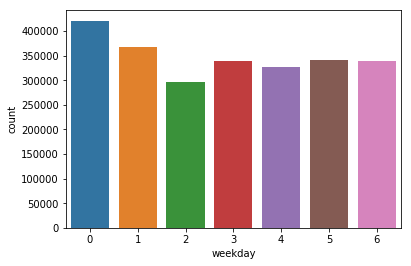
\includegraphics[width=3.5cm]{images/weekday_count.png}}}%
    \qquad
    \subfloat[Hour]{{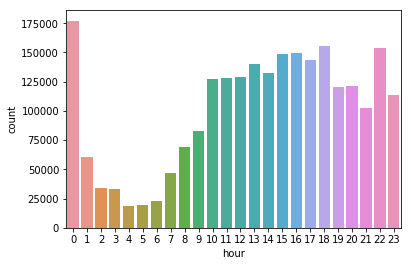
\includegraphics[width=3.5cm]{images/hour_count.png} }}%
    \qquad
    \subfloat[Advertiser]{{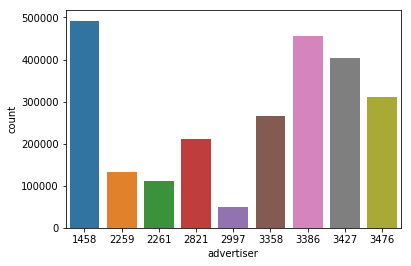
\includegraphics[width=8cm]{report/images/advertiser_count.png} }}%
    \qquad
    \subfloat[OS]{{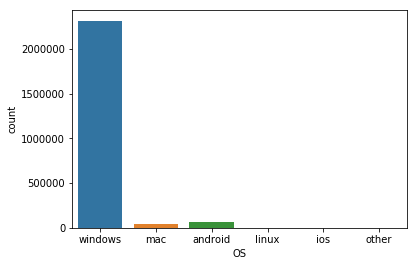
\includegraphics[width=8cm]{report/images/os_count.png} }}%
    \qquad
    \subfloat[Browser]{{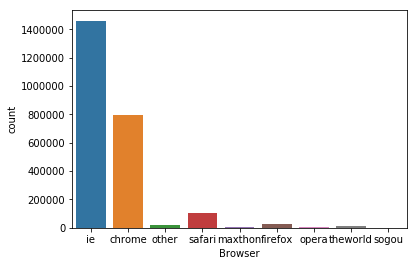
\includegraphics[width=8cm]{images/browser_count.png} }}%
    \caption{User Feedback}%
    \label{fig:user-feedback}%
\end{figure}

\begin{figure}[h!]
	\centering
	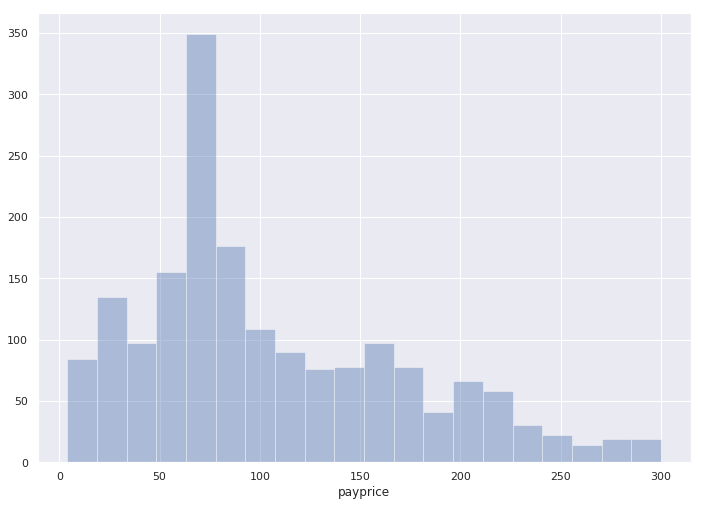
\includegraphics[width=\linewidth]{images/payprice_click_dist.png}
	\caption{Distribution of payprices for clicked impressions}
	\label{fig:click-payprice-dist}
\end{figure}


\section{Approach and Results}
% the approach and result section gives your answers to each of the specific questions and provide the evaluation results and your discussions. 
In this section, we discuss the approaches taken to implement different bidding strategies. For all the approaches, we work with a budget of 6,250 CNY fen to maximise the number of click impressions from the validation dataset, containing 303,375 impressions.

In addition, depending on the scenario, the winning criterion used will different/differ. This is shown in Table \ref{table:winning-criterion}. 

\begin{table}[h!]
  \centering
	\caption{Overview of Winning Criterion}
	\label{table:winning-criterion}
	    \scalebox{0.85}{
		\begin{tabular}{c c c}
			\hline
			Criterion & Scenario & Condition\\
			\hline
			1 & Single Agent &  bid $\geq$ payprice \\
			2 & Multi Agent &  bid $\geq$ payprice \& otherSubmittedBids \\
			\hline
		\end{tabular}
		}
\end{table}

\subsection{Basic Bidding Strategies}
For basic bidding strategies, they do not depend on the many features provided in each impression. They are simply determined by basic information such as the agent's budget, impression prices and total impressions up for bid.

\subsubsection{Constant Bidding Strategy}
In a constant bidding strategy, a constant bid is chosen and applied regardless of the information provided in every impression. For this strategy, we will be working in a single-agent environment using winning criterion 1. 

To obtain the optimal constant value, we set bid prices from 1 to 200 and validate the performance. The results are illustrated in Figure \ref{fig:const-clicks} where we observe that the performance improves linearly with bid prices till it reaches a peak at 77 before falling off. Table \ref{table:const-result} shows the top 3 results obtained from our constant bidding finding.

\begin{figure}[h!]
    \centering
    %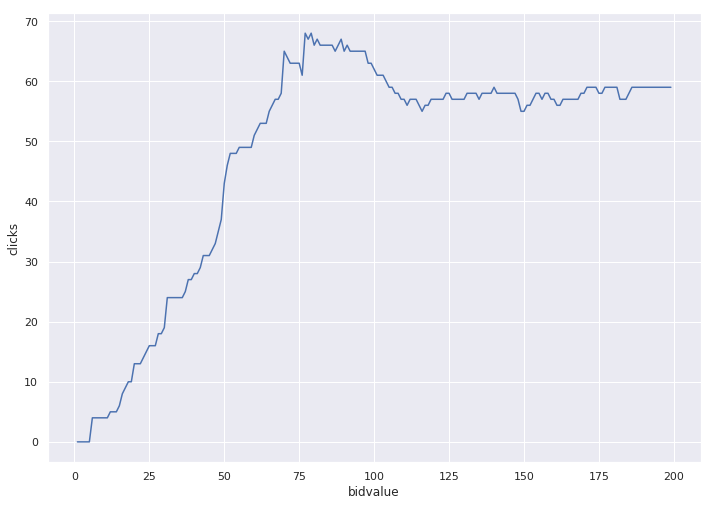
\includegraphics[scale=0.3]{images/const_bid.png}
    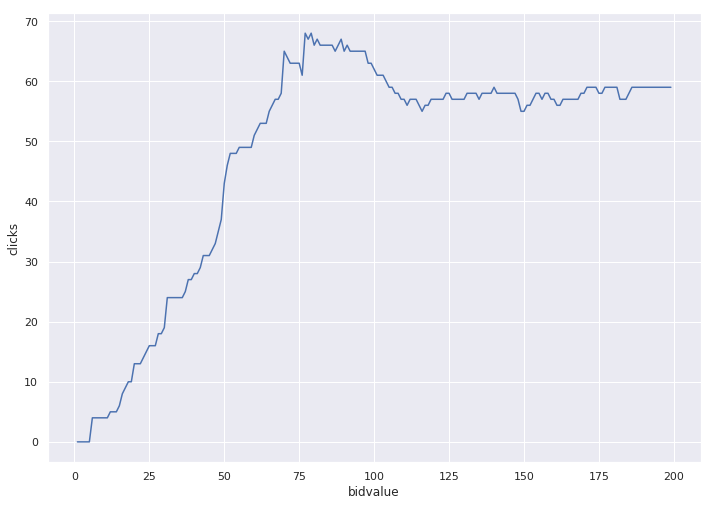
\includegraphics[width=\linewidth]{images/const_bid.png}
    \caption{Clicks at different constant bid prices}
    \label{fig:const-clicks}
\end{figure}

\begin{table}[ht]
  \centering
	\caption{Constant Bidding Results}
	\label{table:const-result}
		\begin{tabular}{c c c c c c}
			\hline
			Click & Range & Imps & CTR & CPC & Spent \\
			\hline
            68 & 77 & 146,864 & 0.00046 &	91.91 & 	6,249.99 \\
           	68 & 79 & 145,916 & 0.00047 &	91.91 & 	6,249.99 \\
            67 & 78 & 146,311 & 0.00046 &	93.28 & 	6,249.99 \\
            \hline
		\end{tabular}
\end{table}
 
\subsubsection{Random Bidding Strategy}\label{rand-bidding}
In a random bidding strategy, bids are randomly selected from within a certain range. We empirically determine this optimal range under winning criterion 1 by testing it against the validation dataset. To account for the random nature of the bids, 10 sets of bids are generated for every range and we take the average performance from them.

\begin{table}[h]
  \centering
	\caption{Random Bidding Results}
	\label{table:rand-result}
        \scalebox{0.95}{
		\begin{tabular}{c c c c c c}
			\hline
			Click & Range & Imps & CTR & CPC & Spent \\
			\hline
            55.7 & {[1, 300]}   & 100,911.1 & 0.00055 &	112.20     & 	6,249.96 \\
            61.9 & {[1, 150]}   & 137,880.7 &	0.00045 &	100.96 & 6,249.97 	\\
            55.1 & {[150, 300]} & 87,857.7  &	0.00063 &	113.42 & 6,249.93 \\
			\hline
            67.6 & {[50, 100]} & 151,761.3 &	0.00045 & 92.45  & 6,249.97 	\\
            64.8 & {[75, 80]}  & 149,350.8 & 0.00043 & 96.45  & 6,249.96 \\
            57.7 & {[75, 150]} & 120,793.7 &	0.00048 & 108.31 & 6,249.96 \\
            47.9 & {[1, 100]}  & 116,589.2 &	0.00041 & 87.52  & 4,192.38 \\
            29.9 & {[1, 75]}   & 84,554.8  &	0.00035 & 76.81  & 2,296.67	\\
			\hline
		\end{tabular}}
\end{table}

Table \ref{table:rand-result} shows the results of the tested ranges. The ranges $[1, 300]$, $[1, 150]$ and $[150, 300]$ were used to covers all possible bids in the validation set dataset and generate a baseline performance of around 55.7 clicks. It also showed that the optimal range would be located in lower half of the bid range.

Focusing on the lower half of the bids, it was found that the best performing range was between 50 to 100 with an average of 67.6 clicks. This result was further supported by the payprice distribution we saw in Figure \ref{fig:click-payprice-dist}, where most clicked impressions had a payprice of under 100. 

\subsubsection{Homogeneous Random Bidding Agents} \label{homogeneous-agents}
We next look at how the environment changes with the introduction of multiple bidding agents using winning criterion 2. 

With the introduction of multiple agents, the auction environment becomes more complex where every agent's bids affects the final payprice and individual agent's budgets have to be accounted for. Since we are using homogeneous agents, we expect every agent to achieve similar performances.

Table \ref{table:rand-homo-result} shows our test results. We first used the single agent optimal random bidding range (50-100) and tested it against 50, 75 and 100 homogenous agents. As expected, the average agent's performance was much lower compared to the single agent environment where clicks dropped from 67.6 to around 1-3 clicks. Also, we found that the average number of clicks, impressions and budget spending reduces with increasing number of agents, in fact, none of the agents went out of budget (OOB) in our tests.

We then tested a high bid range (300-350) that guarantees winning of all available impressions in the dataset. We observe that the average performance of all agents has improved, but even then, none of the agents went out of the budget.

Finally, we tested with a narrow bidding range (300-310) and found that even though the average performance was similar, some agents performed much better and went out of the budget. We found that because of the narrower range, it increased the odds of similar bids where the simulation environment simply awards it to the first agent. Since the bidding order is always the same, some agents therefore get an inherent advantage to win over others, thereby creating this disparity.

From our results, in a multi-agent environment, it is possible for all agents to win every impression without exhausting their budget. But this is only when the win probability of all agents are even. So in an optimal homogeneous multi-agent environment, every agent would bid at price ranges that ensures all impressions in the dataset can be won (>300) and set a range large enough such that every agent has an equal probability of winning.

\begin{table}[ht]
  \centering
	\caption{Performance of different agent counts and bids}
	\label{table:rand-homo-result}
		\begin{tabular}{c c c c c c c}
			\hline
             Agents & Range & Click & Imps & Spent & OOB  \\
			\hline
			50 &	[50, 100] & 2.52 &	4553.60 &	668.47 & 0\\
			75 &	[50, 100] & 1.68 & 3037.13 & 447.83  & 0\\
			100 & [50, 100]	& 1.26 & 2278.51 & 336.74  & 0\\
			\hline
            50 & [300, 350] & 4.04 & 6087.50 & 2588.04  & 0\\
            75 & [300, 350] & 2.69 & 4052.33 & 1727.95 & 0 \\
            100 & [300, 350] & 2.02 & 3039.25 & 1296.92 & 0 \\ 
			\hline
            50 & [300, 310] & 4.04 & 6087.50 & 2353.53 & 9 \\
            75 & [300, 310] & 2.69 & 4052.33 & 1569.18  & 9\\
            100 & [300, 310] & 2.02 & 3039.25 & 1176.90  & 9\\ 
            \hline
		\end{tabular}
\end{table}


\subsection{Advanced Bidding Strategies}
Next we look into advanced bidding strategies that use CTR estimation models to determine click probability of impressions. These strategies vary the bids such that higher click probabilities will be more aggressively bid for.

\subsubsection {CTR Estimation}
\textbf{Models:}
We considered two different CTR estimation models; Logistic Regression (LR) and Gradient Boosting Regression Tree (GBRT). The first one is a type of probabilistic statistical classification model which uses a binary predictor and the latter is a non-linear model which has the advantage of learning from the continuous features instead of binary features as required in the LR model. For LR, we use the implementation provided by scikit-learn and for GBRT, we use the open source library, XGBoost. 

\textbf{Features:} As mentioned in Table \ref{table:data-format} we selected 14 categorical features from the dataset to be used for training. Additionally, we performed feature engineering on the following 3 fields before applying one hot encoding on them. In total, we have used 606 binary features for the training of our classifier.

\begin{itemize}
    \item useragent: Split into OS and browser details, the original useragent field is removed
    \item slotprices: Labelled into the ranges $[0,10]$, $(10,50]$, $(50,100]$, $(100, 150]$, $(150,+\infty]$
    \item usertag: Split into binary features for each user
\end{itemize}

However, during the training stage we faced two problems. Firstly the imbalance of negative results (99.926\% of training set) caused our resultant models to become improperly trained. Secondly, as we feature engineered and increased the size of our training data, there was a point where our devices were no longer able to load it in memory. Thus, we turned to negative downsampling \cite{he_practical_2014} to solve both problems. 

\textbf{Negative Downsampling:} In negative downsampling, we reduce the negative data from the training set to remove the bias and also reduce the data size of the training data. To determine the best rate to use, we tried different downsampling rates on our models and evaluated them with the widely used, area under ROC curve (AUC) measurement. \cite{ferro_deep_2016, DBLP:conf/icml/GraepelCBH10}. Our results is presented in Figure \ref{fig:downsample-auc-score} where we found that except on the lowest sample rate, GBRT consistently showed better results as compared to LR. So our best performing model is the GBRT model at a downsampling rate of 0.0005, providing an AUC score of 0.7785. The chosen model is then used for subsequent bidding strategies. 
	
\begin{figure}[h!]
	\centering
	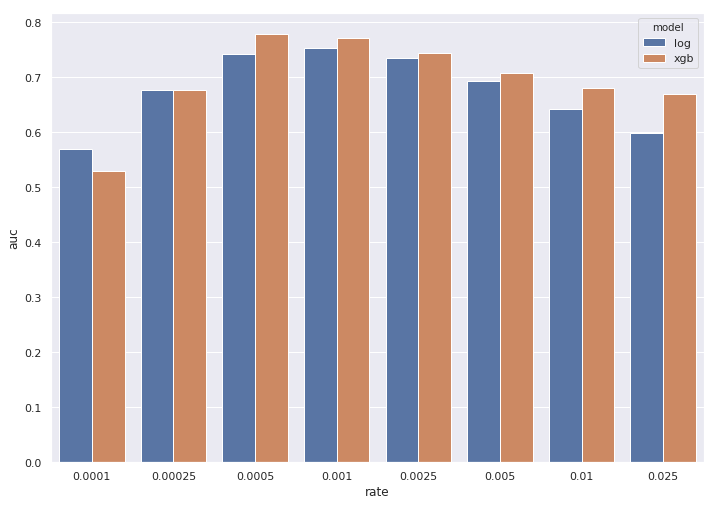
\includegraphics[scale=0.25]{images/model_auc.png}
	%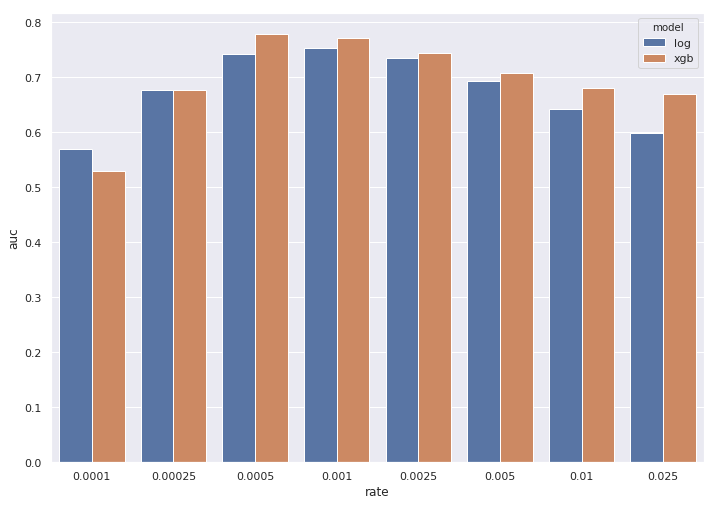
\includegraphics[width=\linewidth]{images/model_auc.png}
	\caption{AUC scores at different downsampling rates}
	\label{fig:downsample-auc-score}
\end{figure}

\textbf{Re-calibration:} Negative downsampling helped improve the model and training times, however, the CTR estimates by the model were also affected by the negative downsampling and cannot be used as it is. A re-calibration formula \ref{eq:recal-downsample} needs to be applied to the model's CTR to get the real predicted CTR \cite{he_practical_2014} by the model.

\begin{equation}\label{eq:recal-downsample}
   \mathrm{CTR}_\mathrm{pred} =  \frac{\mathrm{CTR}_\mathrm{model}}{\mathrm{CTR}_\mathrm{model} + \frac{1 - \mathrm{CTR}_\mathrm{model}}{downsampleRate}}
\end{equation}

\subsubsection{Linear Bidding Strategy}
% Check if citations required for linear bidding
In a linear bidding strategy, the bid values are determined in a linear proportion to the predicted CTR of the impression. Formula \ref{eq:linear-eq} shows how bids are computed in a linear bidding strategy, $\mathrm{CTR}_\mathrm{pred}$ is obtained from the CTR estimation model, whereas $\mathrm{CTR}_\mathrm{avg}$ is obtained from the training dataset. 

\begin{equation} \label{eq:linear-eq}
\mathrm{bid}_\mathrm{value} = \mathrm{bid}_\mathrm{base} * \frac{\mathrm{CTR}_\mathrm{pred}}{\mathrm{CTR}_\mathrm{avg}}  
\end{equation}

We then tune $\mathrm{bid}_\mathrm{base}$ by trying different values to empirically determine the best value. Figure \ref{fig:linear-basebid-tune} shows our observation where our best performing $\mathrm{bid}_\mathrm{base}$ value lies between 124 and 129. Table \ref{table:linear-basebid-tune} shows the top 3 performing base bids from this range, where 129 was our optimal $\mathrm{bid}_\mathrm{base}$.

\begin{figure}[h!]
	\centering
	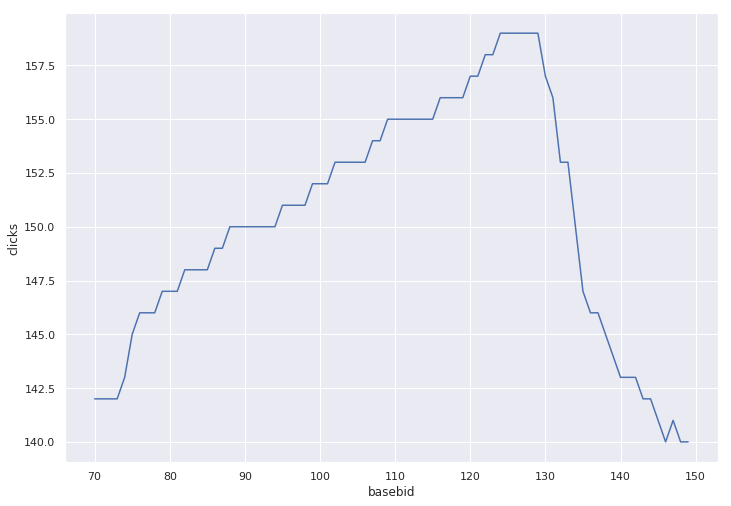
\includegraphics[width=\linewidth]{images/linear_bid_tuning.png}
	\caption{Click results at different base bids}
	\label{fig:linear-basebid-tune}
\end{figure}

\begin{table}[ht]
  \centering
	\caption{Optimal base bid results}
	\label{table:linear-basebid-tune}
		\begin{tabular}{c c c c c c}
			\hline
			Click & $\mathrm{bid}_\mathrm{base}$ & Imps & CTR & CPC & Spent \\
			\hline
            159 & 129 & 138,040 & 0.00115 & 39.31 & 	6,250.00 \\
           	159 & 128 & 137,414 & 0.00116 & 39.03 & 	6,205.56 \\
            159 & 127 & 136,647 & 0.00116 & 38.72 & 	6,156.00 \\
            \hline
		\end{tabular}
\end{table}

\subsubsection{Non-Linear Bidding Strategy}
In a non-linear bidding strategy, the bid values are determined in a non-linear relationship with the predicted CTR of an impression. We implement 2 different Optimal Real-Time Bidding (ORTB) strategies \cite{zhang_optimal_2014} and evaluate the best performing results they get in our dataset.

Formulas \ref{eq:ortb1} and \ref{eq:ortb2} below shows the 2 bidding functions in ORTB, the equations uses the predicted CTR from our CTR estimation model and tuning parameters $c$ and $\lambda$ which are determined empirically from the dataset.

\begin{equation} \label{eq:ortb1}
\mathrm{bid}_\mathrm{ortb1} = \sqrt{\frac{c}{\lambda}*\mathrm{CTR}_\mathrm{pred} + c^{2}} - c
\end{equation}

{\tiny
\begin{multline} \label{eq:ortb2}
    \tiny{\mathrm{bid}_\mathrm{ortb2}} =  \\
    c * [ (\frac{\mathrm{CTR}_\mathrm{pred} + \sqrt{c^{2}\lambda^{2} + \mathrm{CTR}_\mathrm{pred}^{2}}}{c\lambda})^{\frac{1}{3}} - 
    (\frac{c\lambda}{\mathrm{CTR}_\mathrm{pred} + \sqrt{c^{2}\lambda^{2} + \mathrm{CTR}_\mathrm{pred}^{2}}})^\frac{1}{3} ]
\end{multline}
}

We used different combinations of the 2 tuning parameters $\lambda$ ($1e^{-7}-1e^{-5}$) and $c$ ($10-150$) to find our optimal results. Tables \ref{table:ortb1-performance} and \ref{table:ortb2-performance} shows our best performing configurations for the respective ORTB bidding strategies. 

\begin{table}[h!]
  \centering
	\caption{ORTB 1 Performance}
	\label{table:ortb1-performance}
        \resizebox{\linewidth}{!}{
		\begin{tabular}{c c c c c c c}
			\hline
			Click & $c$ & $\lambda$ & Imps & CTR & CPC & Spent \\
			\hline
            158 & 100 & $2.0e^{-6}$ & 144,609 & 0.00109 & 39.56 & 6,249.97 \\
           	158 & 95 & $2.0e^{-6}$ & 144,342 & 0.00109 & 39.20 & 6,193.43 \\
            156 & 90 & $2.0e^{-6}$ & 143,160 & 0.00109 & 39.12 & 6,103.36 \\
            \hline
		\end{tabular}}
\end{table}

\begin{table}[h!]
  \centering
	\caption{ORTB 2 performance}
	\label{table:ortb2-performance}
        \resizebox{\linewidth}{!}{
		\begin{tabular}{c c c c c c c}
			\hline			Click & $c$ & $\lambda$ & Imps & CTR & CPC & Spent \\
			\hline
            160 & 150 & $3.4e^{-6}$ & 141,861 & 0.00113 & 38.59 & 6,174.66 \\
           	155 & 90 & $3.0e^{-6}$ & 143,269 & 0.04173 & 38.57 & 5,978.37 \\
            152 & 70 & $2.5e^{-6}$ & 149,213 & 0.00102 & 41.12 & 6,249.97 \\
            \hline
		\end{tabular}}
\end{table}

In terms of clicks, the ORTB strategies were comparable to the linear strategy ($\pm$ 1 click), however ORTB was more efficient with the budget and were able to win more impressions (ortb1: $+$6,569, ortb2: $+$3,821) using the same budget. 

\subsection{Multi-agent Bidding Strategy}
Finally, we look at how the different strategies work in a multi-agent environment. We put all 5 different optimal strategies discussed above together in a winning criterion 2 auction to see how they perform. The results as seen in Table \ref{table:strategies-compared} shows that surprisingly, our best performing single-agent strategy, ORTB2, performed badly with only 30 clicks. ORTB1 and linear bidding performed best with 63 clicks and 62 clicks respectively. ORTB1 also had the best CTR and CPC to achieve the best performance while spending only 2744.33. It looks to be the best strategy to implement for our multi-agent strategy.

However as mentioned in section \ref{homogeneous-agents}, given the limited number of impressions, the environment changes with the addition of multiple agents. So to more closely recreate the final environment of 29 groups, we look to optimise the strategies using 30 agents, using 6 agents for each strategy mentioned above. In this case, the linear bidding strategy dominated and won most of the click impressions. From this, we determine that ORTB1's performance earlier was likely due to it performing well after the linear strategy ran out of the budget, but since there are more agents to carry on the linear strategy, ORTB1 did not have a chance. 

\begin{table}[h]
  \centering
	\caption{Strategies compared}
	\label{table:strategies-compared}
        \resizebox{\linewidth}{!}{
		\begin{tabular}{c c c c c c c}
			\hline
			Strat & Click & Imp & CTR & CPC & Spent & OOB \\
			\hline
			\multicolumn{7}{c}{5 Agents - 1 agent per strat}\\
			\hline
            ortb1  & 63 & 16,112 & 0.003910 & 43.56& 2,744.33& 0 \\
            linear  & 62 & 26,938 & 0.002302 & 100.80& 6,250.10& 134,106 \\
            ortb2  & 29 & 38,766 & 0.000748 & 215.52& 6,250.24& 293,019 \\
            const & 7 & 72,953 & 0.000096 & 892.87& 6,250.09& 262,310 \\
            rand  & 2 & 53,419 & 0.000037 & 3,125.05& 6,250.11& 211,173 \\
            \hline
			\multicolumn{7}{c}{30 agents - 6 agents per strat - Top 5}\\
			\hline
            linear_4  & 48  & 18,591  & 0.002582  & 130.22& 6,250.71& 290,984 \\
            linear_0  & 45  & 18,427  & 0.002442  & 138.89& 6,250.12& 96,126 \\
            linear_3  & 42  & 18,295  & 0.002296  & 148.81& 6,250.15& 192,926 \\
            linear_5  & 11  & 2,459  & 0.004473  & 72.68& 799.51& 0 \\
            rand_5  & 8  & 29,223  & 0.000274  & 481.70 & 3,853.58& 0 \\
			\hline

		\end{tabular}}
\end{table}

Though ORTB1 was more efficient, it was too conservative in a multi-agent setting and it gets outbid in the presence of multiple aggressive bidders. So we tried making it more aggressive by combining both linear and ORTB1 as shown in formula \ref{eq:ortb1-linear}. The strategy makes it bid more aggressively when confident and less aggressively otherwise. We also included a sensitivity constant $c$ to tune the effect of the ratio. Table \ref{table:linear-ortb} shows that by reducing the sensitivity to 0.45, we spent our budget more effectively and got our best performance at 86 clicks. 

\begin{equation} \label{eq:ortb1-linear}
\mathrm{bid}_\mathrm{linORTB1} = c * \frac{\mathrm{CTR}_\mathrm{pred}}{\mathrm{CTR}_\mathrm{avg}} * \mathrm{bid}_\mathrm{ortb1}
\end{equation}

\begin{table}[h]
  \centering
	\caption{Linear ORTB Performance}
	\label{table:linear-ortb}
        \resizebox{\linewidth}{!}{
		\begin{tabular}{c c c c c c c}
			\hline
			Strat & Click & Imp & CTR & CPC & Spent & OOB \\
			\hline
            \multicolumn{7}{c}{31 agents - 6 agents per strat + linORTB1 (c = 1.0)}\\
			\hline
            linORTB1 & 55 & 12,215 & 0.0045 & 113.64& 6,250.26& 128,967 \\
            linear_3 & 48 & 18,588 & 0.0025 & 130.21& 6,250.10& 290,335  \\
            linear_0 & 33 & 24,608 & 0.0013 & 189.59& 6,256.71& 192,339  \\
			\hline
            \multicolumn{7}{c}{31 agents - 6 agents per strat + linORTB1 (c = 1.2)}\\
			\hline
            linORTB1 & 47 & 15,226 & 0.0030 & 132.99& 6,250.58& 109,607 \\
			\hline
            \multicolumn{7}{c}{31 agents - 6 agents per strat + linORTB1 (c = 0.8)}\\
			\hline
            linORTB1 & 63 &9,797 &0.0064 &99.21&6,250.26&154,987 \\
			\hline
            \multicolumn{7}{c}{31 agents - 6 agents per strat + linORTB1 (c = 0.45)}\\
			\hline
            linORTB1 &86 &6,148 &0.0139 &72.69 &6,251.56 &269,478 \\
			\hline
		\end{tabular}}
\end{table}

A supplementary strategy we then considered was to conserve our budget early by bidding less for the first half of the auction, then increasing our bid proportionally in the latter half. The idea is to let the competition tire out before coming in. From our finding in Table \ref{table:budget-conversation}, the original bidding strategy still provided the best results. So we stuck with that for our final multi-agent bidding strategy. 

\begin{table}[h]
  \centering
	\caption{Budget Conservation Performance}
	\label{table:budget-conversation}
        \resizebox{\linewidth}{!}{
		\begin{tabular}{c c c c c c c}
			\hline
			Bid Ratio & Click & Imp & CTR & CPC & Spent & OOB \\
			\hline
            100\% & 86 & 6,148 & 0.0139 & 72.69 & 6,251.56 & 269,478 \\
            90\% / 110\% & 84 & 6,128 &0.0137 &74.40 & 6,250.06 &279,027 \\
            75\% / 125\% & 82 & 6,541 &0.0125 &76.22 & 6,250.09 &300,585 \\
            50\% / 150\% & 79 & 7,723 &0.010229 &76.81 & 6,068.48 &0 \\
			\hline
		\end{tabular}}
\end{table}

\section{Limitation and Future Work}
\textbf{Improve CTR classifiers:}
In our study, we only explored 2 CTR classifiers, LR and GBRT and we focused on feature engineering instead of optimising the classifiers' parameters. Choosing better classifiers or fine tuning existing ones should create a more accurate CTR estimator such that the bidding strategies will be more effective. 

\textbf{Explore other bidding strategies:}
We only managed to explore the non-linear ORTB strategy in our study, however there are other strategies, such as lift-based bidding\cite{xu_lift-based_2015} that was not evaluated. Those strategies could have been possibly be more efficient than the one that was used in our study. With time we would explore further to make a more informed decision on the non-linear strategies to use.

\textbf{Multi-agent strategy:}
In our multi-agent strategy, we created bidding strategies that was more effective against what we have discovered so far. It did not consider changes in strategies that were implemented by other agents. A better way would have been to create a Stochastic game for multi-agent reinforced learning \cite{jin_multiagent_2018} and use the algorithms to create the ideal bidding strategy. 

\section{Conclusion}
% the conclusion section concludes your report and point out the potential direction to improve your report (e.g., if you have time, you will do...).
In this study we explored multiple bidding strategies in both single and multi-agent environments. In the single agent environment, we found that basic bidding strategies produced only limited results as compared to more advanced strategies that uses a CTR estimator. This is seen where our best performing basic bidding strategy only produced 77 clicks as compared to the 160 from our advanced bidding strategy. In the multi-agent environment the strategies that previously worked in a single environment will need to be adapted to handle other agents. We modified our original non-linear ORTB 1 bidding strategy to be more sensitive to handle bids from other agents and achieved the best performing result when compared with 30 other agents in our experimentation. 

\clearpage
\newpage
\bibliographystyle{abbrv}
\bibliography{ref}  

\end{document}